\section{Metalle}
Typische Eigenschaften: gute elektrische und Wärme-Leitfähigkeit, Duktilität, Glanz \\

\subsection{Elektronengas-Modell}
Metallkationen bilden ein Gitter, die VE sind delokalisiert (frei beweglich), weil Metalle kleine $E_{Ion}$ haben. \\

Metallische Bindung: ungerichtete elektrostatische Anziehung zwischen Metallkationen und $e^-$-Gas. \\

\subsection{Duktilität}
Reine Metalle sind relativ duktil, weil dichtest gepackte Schichten gut gegeneinander beweglich sind. Duktilität ist abhängig von der Zahl der Gleitebenen (d.h. Gittertyp, Korngrösse), der Stärke der metall. Bindung und der Gitterfehler. 

\subsection{Eisen}
\subsubsection{Aufbau}
\begin{figure}[htbp]
	\centering
	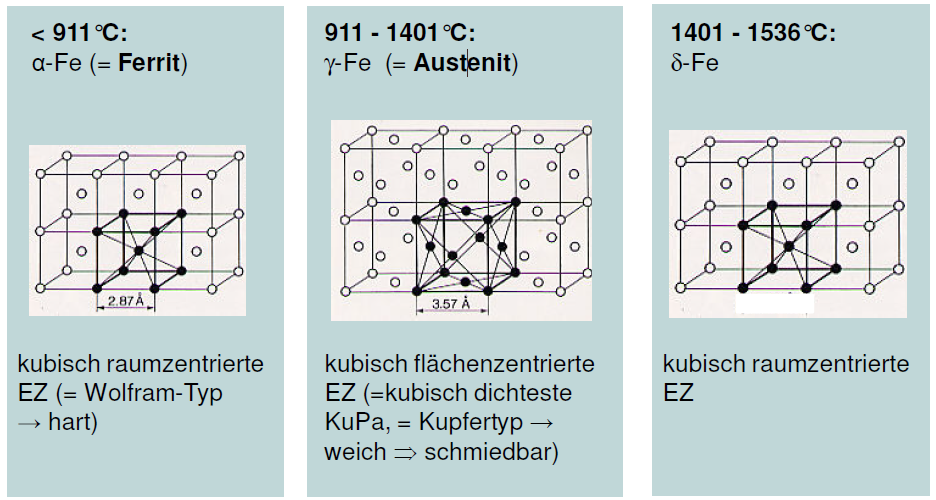
\includegraphics[width=0.9\linewidth]{images/3_Aufbau_Eisen.png}
\end{figure}

\subsection{Energiebänder-Modell}
Überlappung von $N$ Atomorbitalen (AO) führt zu N Molekülorbitalen (MO). Wenn N sehr gross $\Rightarrow$ Bänder aus MO $\Rightarrow$ elektrisch leitend.
\begin{itemize}
	\item Metalle: leeres Leitungsband überlappt mit (teilweise) gefülltem Valenzband
	\item Isolatoren: Grosse verbotene Zone zwischen Valenzband und Leitungsband
	\item Eigenhalbleiter: Kleine verbotene Zone
\end{itemize}

\subsubsection{Eisengewinnung}
Ausgangsstoffe: Fe-Erz, Koks, Zuschlagsstoffe (Kalk, Sand), Luft (O$_2$) \\

Prinzip: $Fe_xO_y + C \leftarrow Fe + CO_2$ \\

Gase: Durch Zuschlagsstoffe gebundene, unerwünschte Erze. \\
Gichtgas: Gase und Rest des Heisswinds. \\

Hochofenprozesse:
\begin{eqnarray*}
	C_{s} \quad &+ O_{2(g)} \quad &\rightarrow \quad CO_{2(g)} \\
	CO_{2(g)} &+ C_{(s)} & \rightarrow 2 CO_{g} \\
	Fe_2O_{3(s)} &+ 2 CO_{(g)} & \rightarrow 2 Fe_{(s)} + 2 CO_{2(g)} 
\end{eqnarray*}

\subsection{Legierungen}
Stoffe, die aus zwei oder mehr Elementen bestehen und metallische Eigenschaften aufweisen.

\begin{itemize}
	\item Substitutionslegierungen: gewisse Gitterplätze sind durch Fremdatome belegt. ($r_\text{Fremdatom} \approx r_\text{Basismetall}$). z.B. Ag-Au-Legierung, Cu$_3$Au
	\item Einlagerungslegierung: gewisse Gitterlücken sind durch Fremdatome belegt. ($r_\text{Fremdatom} \ll r_\text{Basismetall}$). z.B. Stahl, Zementit Fe$_3$C
\end{itemize}

\subsubsection{Eigenschaften}
\begin{itemize}
	\item Härte: Legierungen sind härter als reine Metalle. Ursache: Fremdatome behindern Gleitebenen.
	\item El. Leitfähigkeit: schlechtere leitend als Metalle. Ursache: Fremdatome behindern $e^-$-Fluss.
	\item Korrosionsbeständigkeit: meist korrosionsbeständiger als Metalle.
\end{itemize}

\subsection{Stahl}
\subsubsection{Frischen}
Verfahren zur Reduktion von C im Roheisen durch Einblasen von Sauerstoff. \\
Reaktionen:
\begin{eqnarray*}
	2 Fe + O_2 \quad &\rightarrow 2 FeO \\
	Mn + FeO &\rightarrow MnO + Fe \\
	Si + 2 FeO &\rightarrow SiO_2 + 2 Fe \\
	C + FeO &\rightarrow CO_{(g)}
\end{eqnarray*}

Je höher der C-Gehalt, desto fester und härter, aber spröder. Max. 2.06\% C ist in Eisen löslich. 

\subsubsection{Zusammensetzung}
Legierter Stahl enthält Fremdatome:

\begin{figure}[htbp]
	\centering
	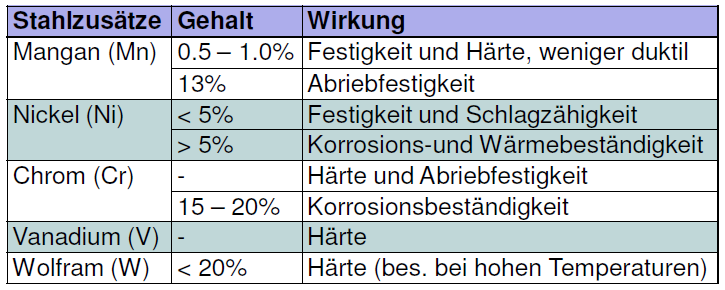
\includegraphics[width=0.9\linewidth]{images/3_Stahl_Zusaetze.png}
\end{figure}

\subsubsection{Eisen-Kohlenstoff-Zustandsdiagramm}
\begin{figure}[htbp]
	\centering
	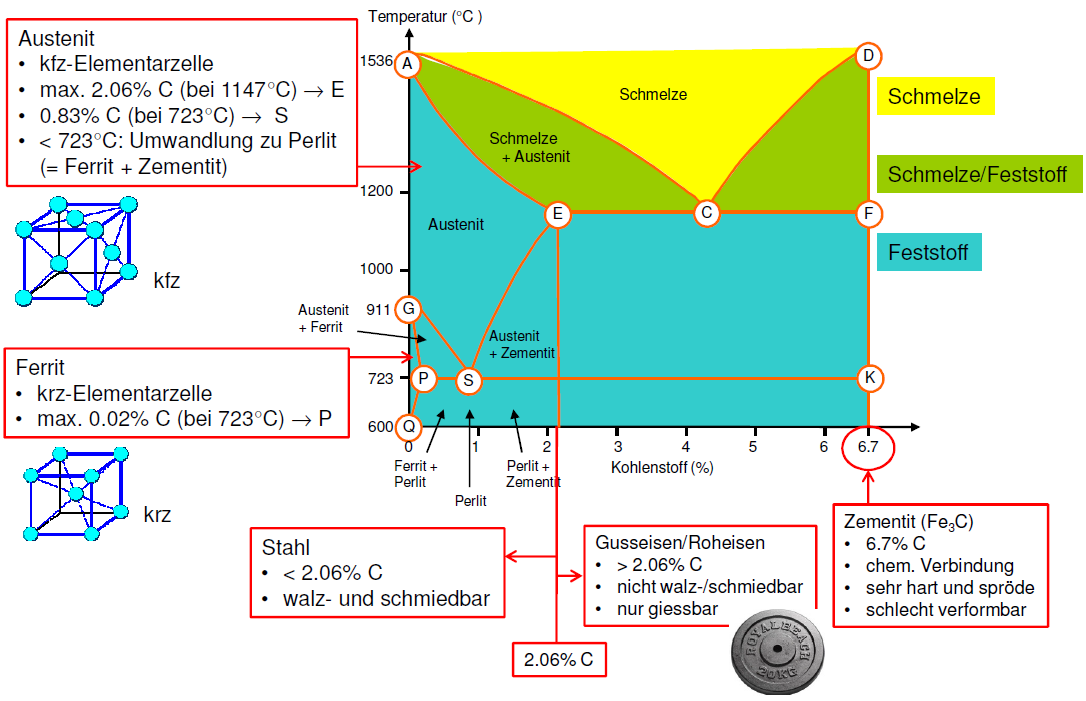
\includegraphics[width=0.95\linewidth]{images/3_Eisen_Kohlenstoff_Diagramm.png}
\end{figure}
